\scanpage{3}
\mspage{2}
is closed nowhere dense in $X_i$, by a) b) c)) \deleted{\unsure{is}} $\operatorname{int}(X_i)=X_i\setminus\partial X_i$, which is therefore a dense \inserted{relatively} open subset of $X_i$, and nonempty since $X_i$ is) is \deleted{\unsure{a}} 1\textsuperscript{o}) \uuline{manifold} 2\textsuperscript{o}) \uline{connected}. (NB in the case of tame $E$, we take ``manifold'' in the tame sense, of course.)
% slanted
\margin{e) If $\deleted{X_i<X_j}\inserted{i<j}$ then $\dim\unsure{\text{the interior}|\operatorname{int}|\operatorname{ind}}(X_i)<\dim\unsure{\operatorname{int}|\operatorname{ind}}(X_j)$, to avoid phenomena of wildness}
% slanted; orient the marginal drawing as on the sheet
\figure{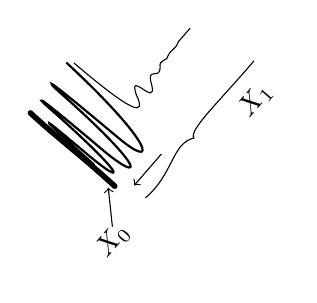
\begin{tikzpicture}[x=.85cm,y=.85cm]
\begin{scope}[rotate=49]
\draw[line width=2pt,line cap=round] (0,0) .. controls (.02,.7) and (-.02,1.15) .. (0,1.67);
\draw[line width=.8pt] (.04,.44) .. controls (.055,1.57) and (.075,1.67) .. (.09,.68)
 .. controls (.10,-.20) and (.23,-.04) .. (.24,1.60)
 .. controls (.26,1.87) and (.28,1.30) .. (.29,.49)
 .. controls (.31,-.34) and (.51,-.17) .. (.52,1.64)
 .. controls (.54,1.88) and (.56,1.58) .. (.58,.46)
 .. controls (.59,-.35) and (.86,-.05) .. (.92,1.76);
\draw (.99,1.67) .. controls (1.00,.48) and (1.10,.33) .. (1.24,.65)
 .. controls (1.45,1.01) and (1.29,.29) .. (1.50,.57)
 .. controls (1.67,.84) and (1.62,.53) .. (1.78,.65)
 .. controls (1.87,.76) and (1.93,.62) .. (2.00,.68)
 .. controls (2.11,.71) and (2.16,.65) .. (2.25,.70) -- (2.52,.70);
\draw[<-] (.20,-.21) -- (.82,-.21);
\draw (.17,-.46) .. controls (.72,-.54) and (1.05,-.22) .. (1.32,-.42)
 .. controls (1.34,-.28) and (2.00,-.35) .. (2.78,-.34);
\draw[->] (-.48,-.37) -- (-.08,.06);
\node[rotate=49] at (-.63,-.51) {$X_0$};
\node[rotate=49] at (2.35,-.74) {$X_1$};
\end{scope}
\end{tikzpicture}}

\deleted{\unsure{e}}f) $X_i\cap X_j$ is a union \unsure{of|of the} $X_k$.

Thus a figure \inserted{$F$} can be identified with the set of its strata, which is a set of closed subsets of $X$
\[
\underset{\substack{\shortparallel\\\{X_i\}}}{F}\subset\mathcal{P}_f(x)
\qquad \text{i.e.}\qquad F\in\mathcal{P}(\mathcal{P}_f(X))
\]
($X$ is reconstituted as $\bigcup X_i$), satisfying certain conditions \inserted{(which we have just made explicit, a) to d))}. We thus have the set of figures, \deleted{which} say $\mathcal{F}$, which is therefore a set of subsets of $\mathcal{P}_f(x)$
\[
\mathcal{F}\subset\mathcal{P}(\mathcal{P}_f)\qquad\text{i.e.}\qquad
\mathcal{F}\in\mathcal{P}(\mathcal{P}(\mathcal{P}_f(X\unsure{)))|))}
\]

To each $F\in\mathcal{F}$ is associated \uline{the ordered set} $\Sigma_F$ of its strata. The disjoint union
\diagram{\begin{tikzcd}[ampersand replacement=\&,column sep=small,row sep=small]
\Sigma \arrow[d,"{\rule{16mm}{.25pt}}"'] \& {}=\displaystyle\coprod_{F\in\mathcal{F}}\Sigma_F\\
\mathcal{F} \&
\end{tikzcd}}
{\reversemarginpar\margin{the fibers are the $\Sigma_F$}}
\margin{\uline{NB} In the case at hand, we \unsure{to|have} $\Sigma_F\equiv F$, \deleted{\unsure{but have it|but I have} \illegible{1} \unsure{already|said}.}}
can also be identified with the set of pairs $(F,X_i)$, \deleted{$F$ e} where $F$ is a figure and $X_i$ is a stratum of $F$ i.e. $X_i\in F$.
